\ifdefined\ishandout
\documentclass[handout]{beamer}
\else
\documentclass{beamer}
\fi

%\usepackage[frenchb]{babel}
\usepackage[T1]{fontenc}
%\usepackage[utf8]{inputenc}
\usepackage{hyperref}
\usepackage{multirow}
\usepackage{listings}
\usepackage{fancyvrb}
\usepackage{tikz}
\usepackage{framed}
\usepackage{algorithm}
\usepackage{algorithmic}
\usepackage{xcolor}
\usepackage{booktabs}
\usepackage{color, colortbl}
\ifdefined\ishandout
\usepackage{handoutWithNotes}
\fi
\usepackage{slashbox}
\usepackage{amsmath}
\usepackage{bm}
\usepackage{hhline}
\usepackage{pgfplots}
\usepackage{caption}
\usepackage{natbib}
\def\bibfont{\footnotesize}
\def\bibname{}


\usetikzlibrary{shapes.geometric}
\usetikzlibrary{positioning}
\usetikzlibrary{shapes.arrows, chains}
\usetikzlibrary{arrows,calc}
\usetikzlibrary{shapes.multipart}
\usetikzlibrary{matrix}

\usepackage{array}
%\usetheme{Boadilla}
\usetheme[progressbar=frametitle]{metropolis}

\usefonttheme[onlymath]{serif}

\newcommand{\R}{\mathbb{R}}
%\newcommand{\C}{\mathbb{C}}
\newcommand{\N}{\mathbb{N}}
\newcommand{\Z}{\mathbb{Z}}
\newcommand{\E}{\mathbb{E}}
\newcommand{\Var}{\text{Var}}
\newcommand{\Cov}{\text{Cov}}
\ifdefined\ishandout
\pgfpagesuselayout{3 on 1 with notes}[a4paper,border shrink=5mm]
\usecolortheme{dove}
\else
%\usecolortheme{dolphin}
%\usecolortheme{crane}
\fi

\metroset{block=fill}

\lstnewenvironment{codeC}
{ \lstset{language=C,
    otherkeywords={printf,scanf}}
}
{}

\ifdefined\ishandout
\definecolor{mygreen}{rgb}{0,0,0}
\definecolor{mymauve}{rgb}{0,0,0}
\definecolor{myblue}{rgb}{0,0,0}
\else
\definecolor{mygreen}{rgb}{0,0.6,0}
\definecolor{mymauve}{rgb}{0.58,0,0.82}
\definecolor{myblue}{rgb}{0,0,1}

\fi

%% Notes
%\setbeameroption{show only notes}


\definecolor{mygray}{rgb}{0.5,0.5,0.5}

\lstset{ language=Python,%
  backgroundcolor=\color{white},   % choose the background color; you must add \usepackage{color} or \usepackage{xcolor}
  basicstyle=\footnotesize,        % the size of the fonts that are used for the code
  breakatwhitespace=false,         % sets if automatic breaks should only happen at whitespace
  breaklines=true,                 % sets automatic line breaking
  captionpos=b,                    % sets the caption-position to bottom
  commentstyle=\color{mygreen},    % comment style
  deletekeywords={...},            % if you want to delete keywords from the given language
  escapeinside={\%*}{*)},          % if you want to add LaTeX within your code
  extendedchars=true,              % lets you use non-ASCII characters; for 8-bits encodings only, does not work with UTF-8
  frame=tb,	                   % adds a frame around the code
  keepspaces=true,                 % keeps spaces in text, useful for keeping indentation of code (possibly needs columns=flexible)
  keywordstyle=\color{blue},       % keyword style
  otherkeywords={*,...},           % if you want to add more keywords to the set
  numbers=none,                    % where to put the line-numbers; possible values are (none, left, right)
  numbersep=5pt,                   % how far the line-numbers are from the code
  numberstyle=\tiny\color{mygray}, % the style that is used for the line-numbers
  rulecolor=\color{black},         % if not set, the frame-color may be changed on line-breaks within not-black text (e.g. comments (green here))
  showspaces=false,                % show spaces everywhere adding particular underscores; it overrides 'showstringspaces'
  showstringspaces=false,          % underline spaces within strings only
  showtabs=false,                  % show tabs within strings adding particular underscores
  stepnumber=2,                    % the step between two line-numbers. If it's 1, each line will be numbered
  stringstyle=\color{mymauve},     % string literal style
  tabsize=3,	                   % sets default tabsize to 2 spaces
  title=\lstname                   % show the filename of files included with \lstinputlisting; also try caption instead of title
}
%\lstset{language=Python,
% breakatwhitespace=false,         % sets if automatic breaks should only happen at whitespace
%  breaklines=true,                 % sets automatic line breaking
%  captionpos=b,                
%%commentstyle=\itshape\color{mymauve},
%%keywordstyle=\bfseries\color{myblue},
%numbers=left,                    % where to put the line-numbers; possible values are (none, left, right)
%  numbersep=8pt,                   % how far the line-numbers are from the code
%  numberstyle=\tiny\color{mygray}, % the style that is used for the line-numbers
%%  rulecolor=\color{black},         % if not set, the frame-color may be changed on line-breaks within not-black text (e.g. comments (green here))
%  showspaces=false,                % show spaces everywhere adding particular underscores; it overrides 'showstringspaces'
%%  showstringspaces=false,          % underline spaces within strings only
%  showtabs=false,                  % show tabs within strings adding particular underscores
%  stepnumber=2,                    % the step between two line-numbers. If it's 1, each line will be numbered
%%  stringstyle=\color{mygreen},     % string literal style
%  tabsize=2 
%}
\ifdefined\ishandout
\newcommand{\red}{\textbf}
\else
\newcommand{\red}{\textcolor{red}}
\fi
%\newcommand \emph
%Default size : 12.8 cm * 9.6 cm

\newcommand{\tmark}[1]{\tikz[remember picture, baseline=-.5ex]{\coordinate(#1);}}

\definecolor{bluegreen}{RGB}{0,149,182}


%\newcommand{\output}[1]{
\setbeamertemplate{navigation symbols}{}
\newcommand{\bvrb}{\Verb[commandchars=£µ§,formatcom=\color{bluegreen}]}
\newcommand{\footvrb}{\footnotesize\Verb}
\newcommand{\vrbalert}[2][]{\visible<#1>{#2}}
%%% Commande pour les listes/arbres
\newcommand{\mvide}{\nodepart{one} \nodepart{two}}
\newcommand{\tvide}{\nodepart{one} \nodepart{two} \nodepart{three}}
\newcommand{\rref}[1][]{\hfill{\scriptsize\textit{#1}}}
 \bibliographystyle{alpha}

%%Fin des commandes pour les listes/arbres.

\bibliographystyle{apalike}

%%% Paramètres du cours (à régler)
%Numéro du cours
\newcommand{\nb}{1}

\title[Machine Learning]{Machine learning and physical modelling-3}
\author[J. Brajard]{julien.brajard@nersc.no}
\institute[NERSC/SU]{NERSC/Sorbonne University\\
\url{https://github.com/brajard/Geilo-Winter-school}}
\date{21-25 January 2018}
\begin{document}
%%%%%%%%%%%%%%%%%%%%% SLIDES DE TITRE
\begin{frame}
\titlepage
%\centering{
%\url{http://australe.upmc.fr} (onglet EPU-C5-IGE Info Gen)}
\end{frame}

\begin{frame}{Table of contents}
  \setbeamertemplate{section in toc}[sections numbered]
  \tableofcontents[hideallsubsections]
\end{frame}

\section{Machine learning as an emulator}
\begin{frame}{Altimeter data}
\begin{columns}[t]
\column{.5\textwidth}
    \begin{figure}
        \centering
        \caption*{Satellite altimeter}
         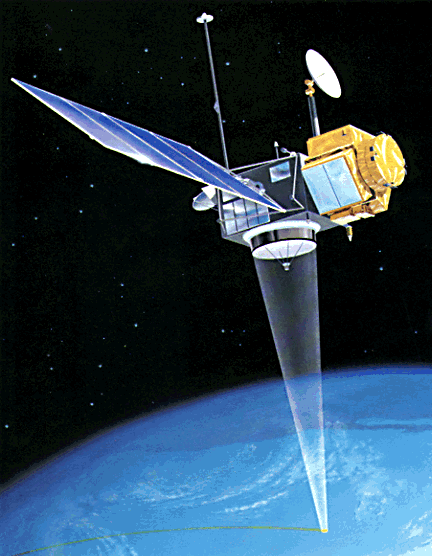
\includegraphics[width=.6\textwidth]{fig/L3/TOPEX-Poseidon.png}
    \end{figure}
    

\column{.5\textwidth}
    \begin{figure}
        \centering
        \caption*{Sea surface height anomaly}
         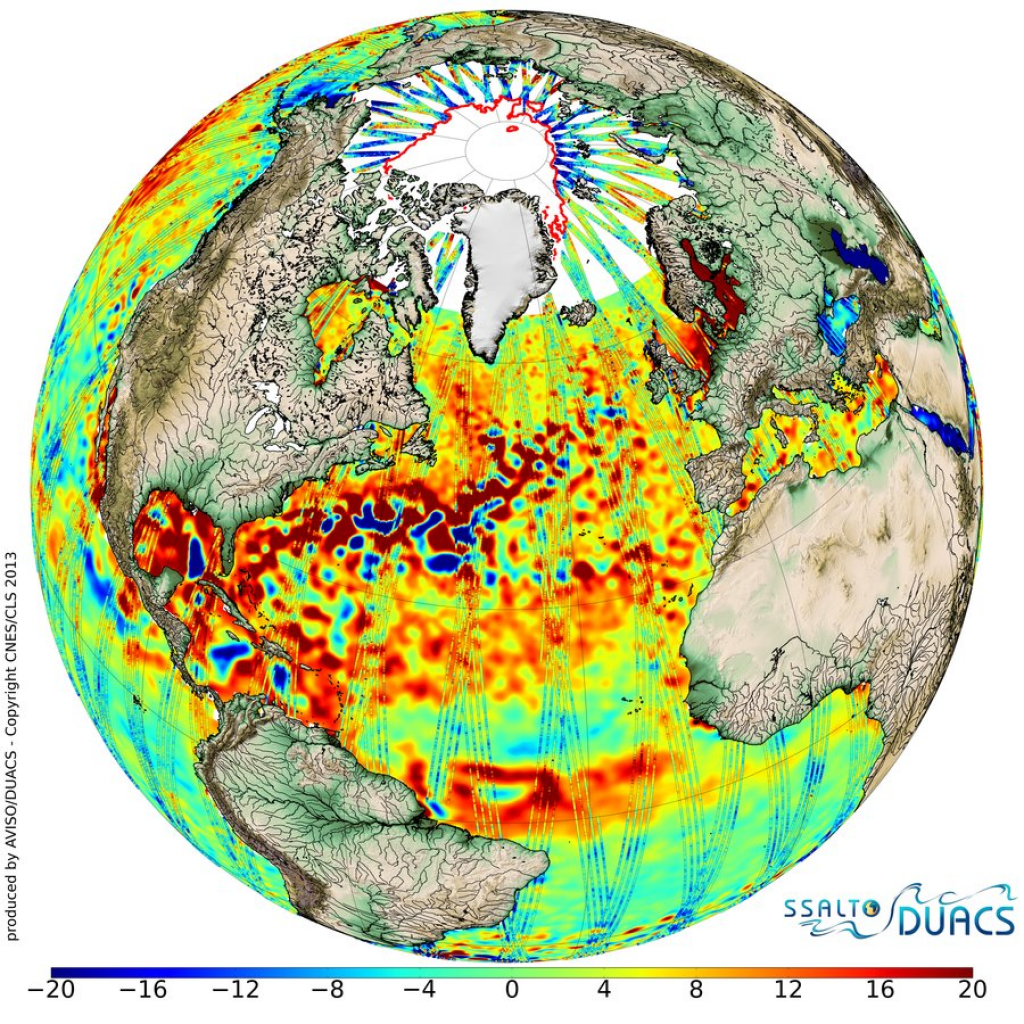
\includegraphics[width=.9\textwidth]{fig/L3/eddies.png}
    \end{figure}

    \end{columns}
    \begin{block}{Structure detection}
    Can we detect and charaterize eddies?
    \end{block}
\end{frame}

\begin{frame}[t]{Eddy detection}
\rref[\cite{Lguensat2017}]
    \begin{columns}
    \column{.65\textwidth}
     \begin{figure}
        \centering
         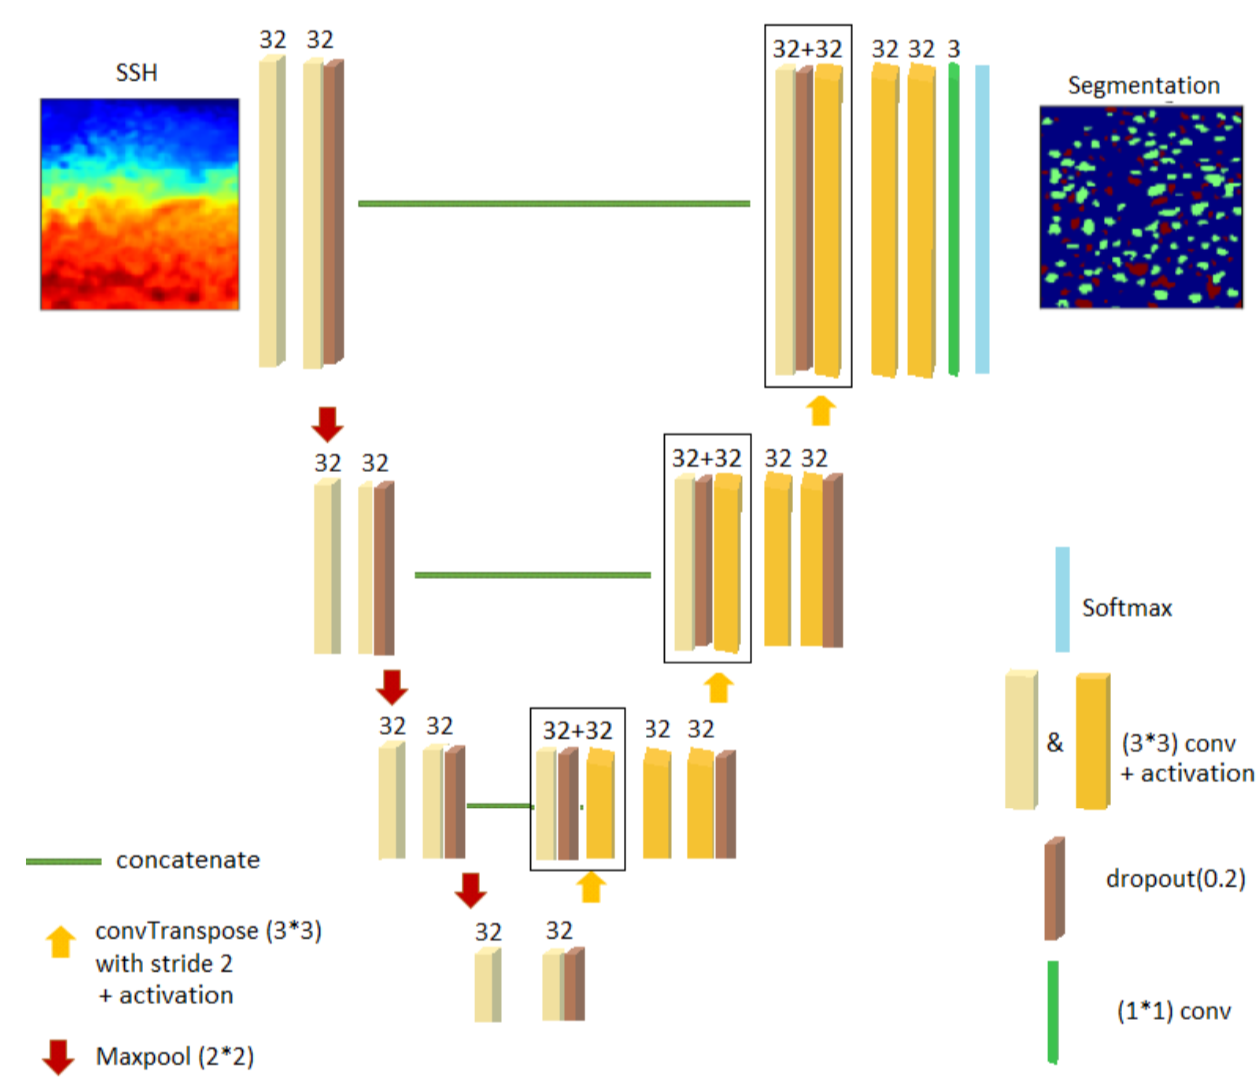
\includegraphics[width=\textwidth]{fig/L3/eddynet.png}
    \end{figure}

    \pause
    \column{.35\textwidth}
         \begin{figure}
        \centering
         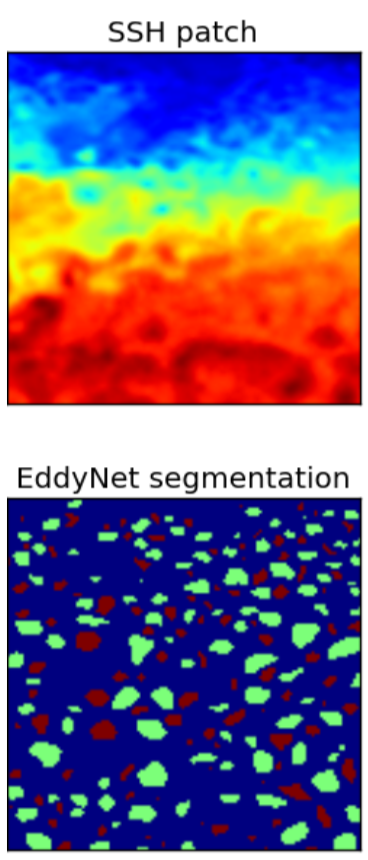
\includegraphics[width=.7\textwidth]{fig/L3/eddynet-result.png}
    \end{figure}
    \end{columns}
\end{frame}

\begin{frame}{Inference of unknown parameters}
    %From Sea Surface Height (SSH) it is also possible to derive (partially) the surface currents.
    \begin{columns}
    \column{.5\textwidth}
          \begin{figure}
        \centering
         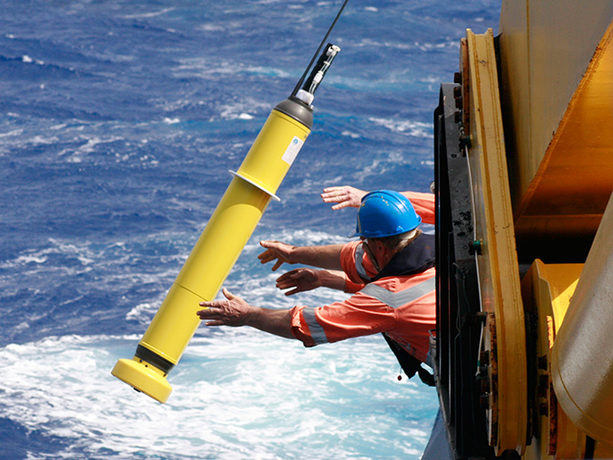
\includegraphics[width=.7\textwidth]{fig/L3/argo-float.jpg}\\
         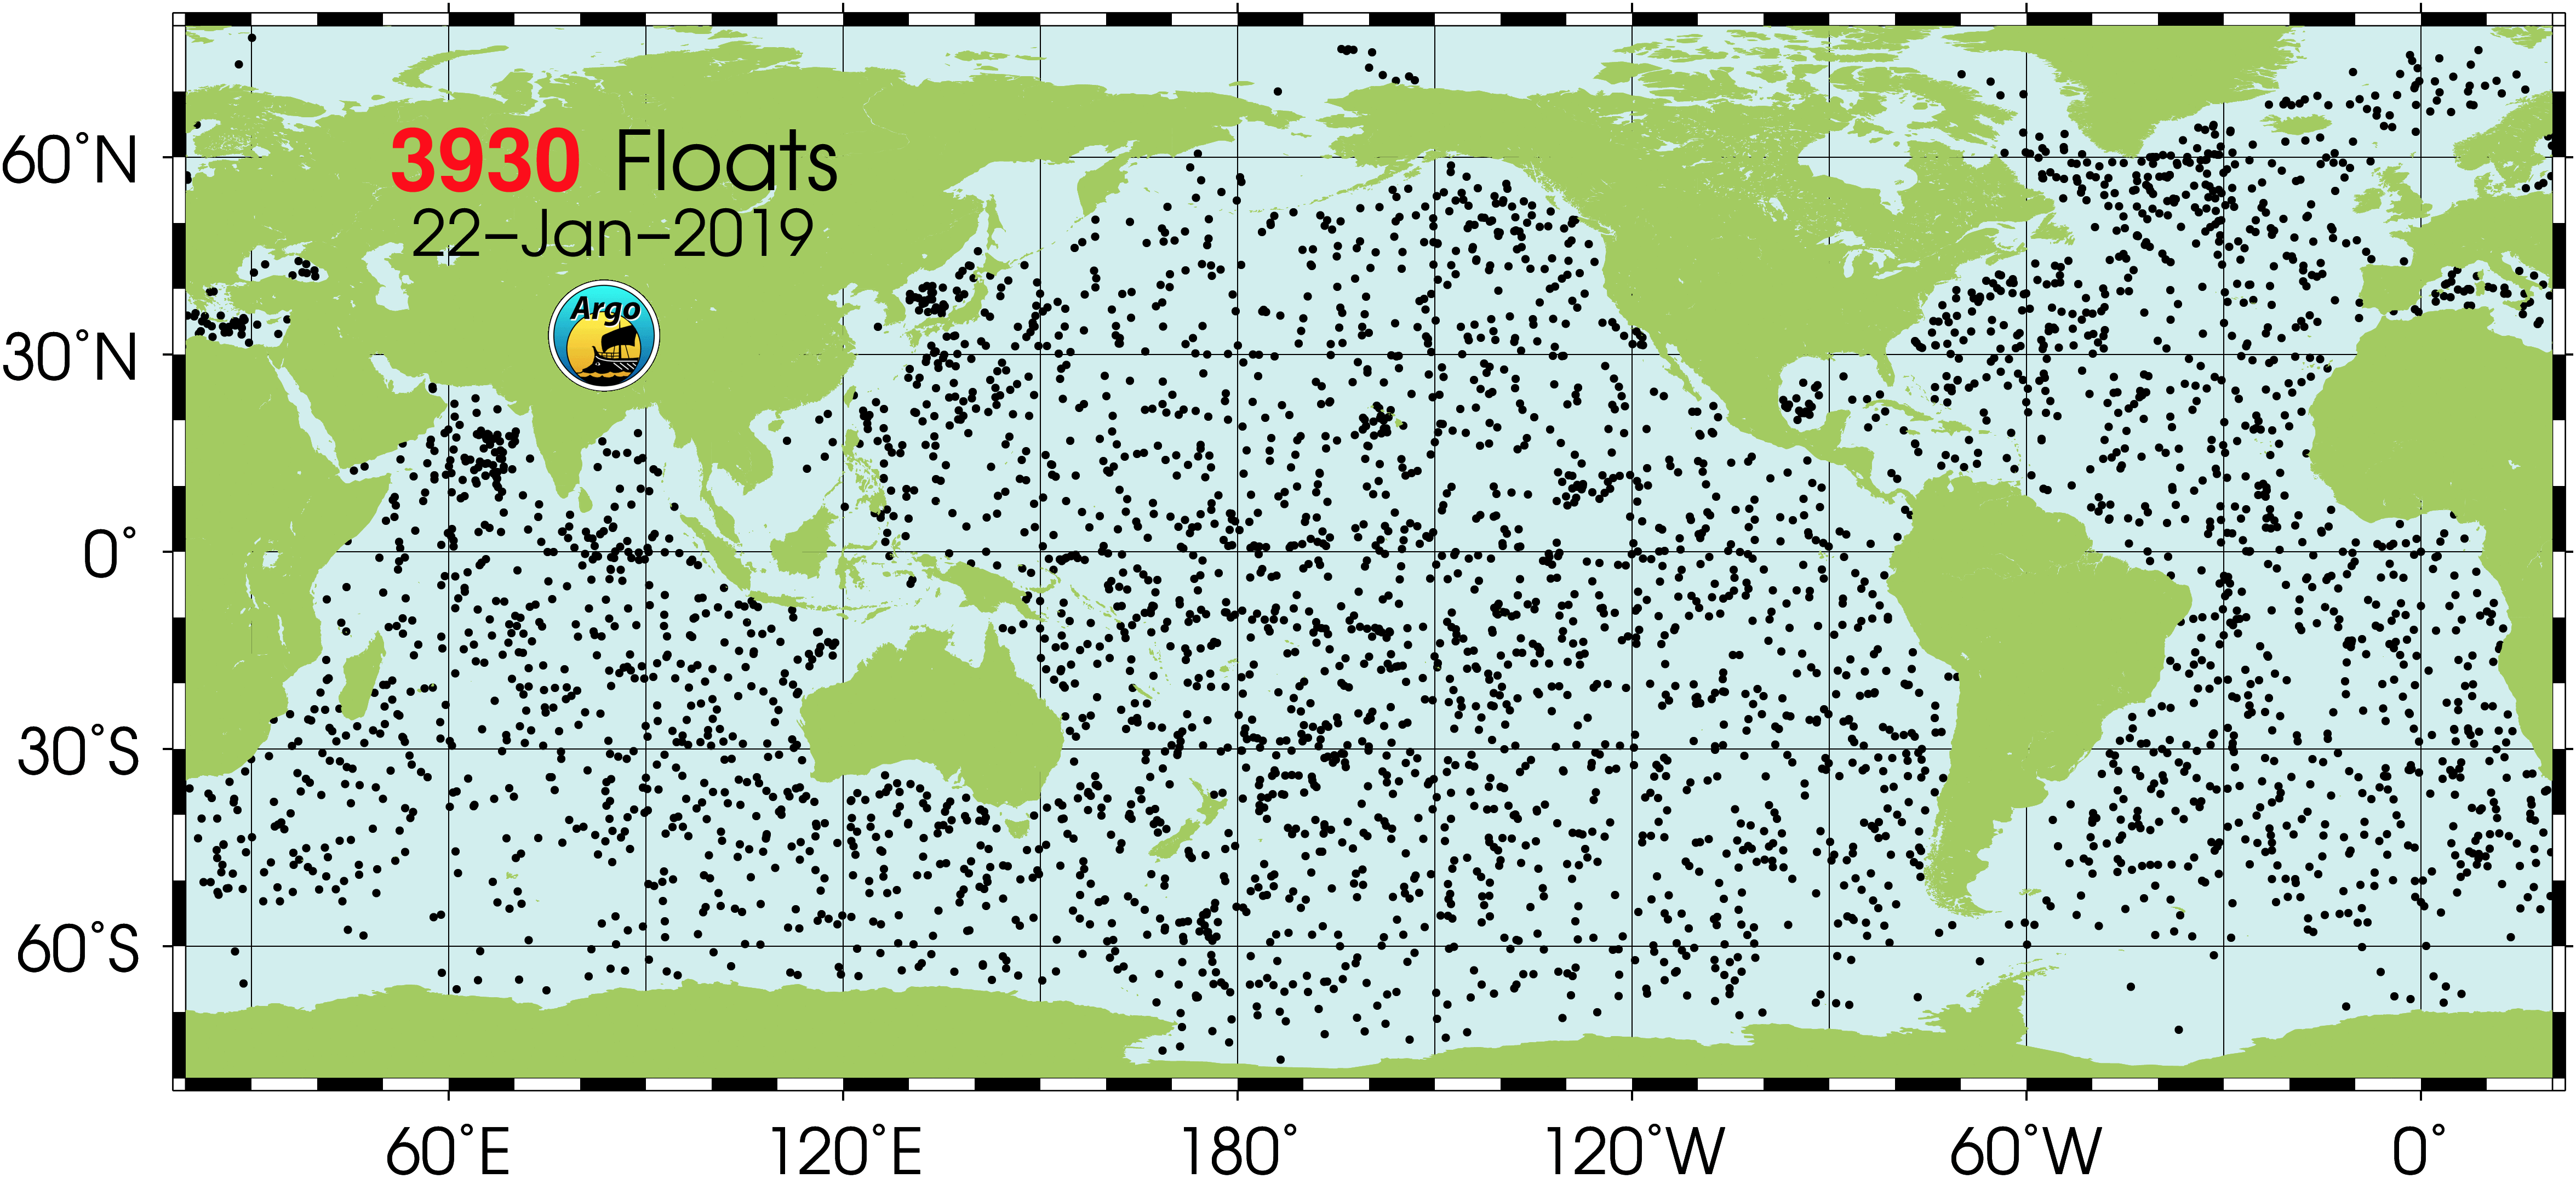
\includegraphics[width=.7\textwidth]{fig/L3/argo-status.png}
    \end{figure}
     \column{.5\textwidth}

    \end{columns}
    \end{frame}
\begin{frame}{Forecasting}
    
\end{frame}
\section{Machine learning and differential equations}
\begin{frame}{phyical system and differential equations}
    
\end{frame}
\begin{frame}{ResNET and ODE}
    
\end{frame}
\begin{frame}{Neural Net integration of ODEs}
    
\end{frame}
\begin{frame}{Toward an unified approach?}
    
\end{frame}
\section{Merge approaches: between physics and machine learning}
\begin{frame}{SST dynamic}
    
\end{frame}
\begin{frame}{Shallow-water and the need of additional constraints}
    
\end{frame}

\begin{frame}{}
   \bibliography{references.bib}
\end{frame}
    
%%%%%%%%%%%%%%%%%%%%%
%%%%%%%%%%%%%%%%%%%%%
%%%%%%%%%%%%%%%%%%%%%
%%%%%%%%%%%%%%%%%%%%%
%%%%%%%%%%%%%%%%%%%%%%%%%%%%%%%%%%%%%%%%%%
%%%%%%%%%%%%%%%%%%%%%
%%%%%%%%%%%%%%%%%%%%%%%%%%%%%%%%%%%%%%%%%%
\end{document}
%%%%%%%%%%%%%%%%%%%%%%%%%%%%%%%%%%%%%%%%%%



